\documentclass[11pt,a4paper]{article}

\usepackage[a4paper,margin=0.8in]{geometry}
\usepackage{booktabs}
\usepackage{longtable}
\usepackage{graphicx}
\usepackage{xcolor}
\usepackage{hyperref}
\usepackage{enumitem}
\usepackage{fancyhdr}
\usepackage{array}

\definecolor{brandgreen}{HTML}{176B57}
\definecolor{lightgreen}{HTML}{EAF5F1}
\definecolor{lightgray}{HTML}{F3F4F6}
\hypersetup{colorlinks=true,linkcolor=brandgreen,urlcolor=brandgreen}
\pagestyle{fancy}
\fancyhf{}
\lhead{Software Engineering Laboratory}
\rhead{Lab 4 - IMG}
\cfoot{\thepage}
\setlength{\headheight}{14pt}

\newcommand{\field}[1]{\rule{0.62\linewidth}{0.4pt}\hfill #1}
\newcommand{\result}[1]{\textcolor{brandgreen}{\textbf{#1}}}

\title{\textbf{Programming Assignment - Real-World Software Applications}}
\author{Software Engineering Laboratory\\Batch IMG}
\date{Experiment 4 \quad | \quad 21 August 2026}

\begin{document}
\maketitle

\begin{center}
\colorbox{lightgreen}{\parbox{0.9\linewidth}{\centering
\textbf{Student submission details}\\[6pt]
Name: \textbf{Nishant Harkut}\\[6pt]
Roll number: \textbf{2023IMG-040}\\[6pt]
Branch: \textbf{IMG}\\[6pt]
Execution date: \textbf{21 August 2026}
}}
\end{center}

\section{Aim}
To design, implement, and test software applications for real-world problems
using appropriate programming concepts and software engineering practices.

\section{Learning Objectives}
\begin{itemize}[leftmargin=*]
  \item Analyze real-world software problems and design a solution before coding.
  \item Implement functional menu-driven console applications.
  \item Apply input validation and error handling.
  \item Test valid, invalid, boundary, and transaction scenarios.
\end{itemize}

\section{Implemented Applications}

\subsection{Hospital Appointment Management System}
The application stores patient records and supports adding, listing, searching,
booking, cancelling, updating, doctor-wise appointment lookup, and appointment
report generation. It validates duplicate and missing patient IDs, empty patient
and doctor names, invalid dates, and appointment state transitions.

\subsection{Restaurant Order Management System}
The application maintains a food catalogue and customer order. It supports food
item management, order add/remove/update operations, subtotal calculation,
discount application, and final bill generation. A 10 percent discount is
applied when the subtotal is at least 1000. Quantities cannot be negative, zero
when adding, or greater than available stock.

\subsection{Vehicle Rental Management System}
The application maintains vehicles and their availability state. It supports
adding, listing, searching, renting, returning, and filtering vehicles. It
rejects duplicate IDs, missing vehicles, empty names, negative prices, renting
an already rented vehicle, and returning an already available vehicle.

\section{Project Structure}
\begin{verbatim}
src/       Application source code and menu entry point
tests/     Unit and console integration tests
data/      Representative JSON input and verified output files
docs/      Test specification, report, and execution screenshots
\end{verbatim}

\section{Testing Summary}

Tests were executed from the repository root using pytest.

\begin{center}
\begin{tabular}{>{\raggedright\arraybackslash}p{0.58\linewidth}r}
\toprule
\textbf{Test area} & \textbf{Result} \\
\midrule
Hospital domain tests & 6 passed \\
Restaurant domain tests & 6 passed \\
Vehicle domain tests & 5 passed \\
Console menu integration test & 1 passed \\
\midrule
Lab 4 total & \result{18 passed} \\
Full semester suite & \result{66 passed} \\
\bottomrule
\end{tabular}
\end{center}

\section{Test Case Report}
\small
\begin{longtable}{p{0.08\linewidth} p{0.28\linewidth} p{0.46\linewidth} p{0.08\linewidth}}
\toprule
\textbf{ID} & \textbf{Scenario} & \textbf{Actual result} & \textbf{Status} \\
\midrule
TC-01 & Valid patient record & Patient added successfully & PASS \\
TC-02 & Duplicate patient ID & Duplicate patient ID error & PASS \\
TC-03 & Invalid appointment date & Date validation error & PASS \\
TC-04 & Appointment already booked & Booking rejected & PASS \\
TC-05 & Valid food item & Food item added successfully & PASS \\
TC-06 & Duplicate food ID & Duplicate food ID error & PASS \\
TC-07 & Quantity greater than stock & Stock validation error & PASS \\
TC-08 & Discount boundary bill & Correct subtotal, discount, and total & PASS \\
TC-09 & Rent available vehicle & Vehicle marked rented & PASS \\
TC-10 & Rent already rented vehicle & Rental state error & PASS \\
TC-11 & Return available vehicle & Return state error & PASS \\
TC-12 & Invalid menu or numerical input & Input rejected with error message & PASS \\
\bottomrule
\end{longtable}
\normalsize

\section{Execution Evidence}

The following pages show the verified output of each menu-driven application.
The corresponding plain-text outputs are stored in 
\texttt{data/output/}.

\clearpage
\vspace*{0.25in}
\noindent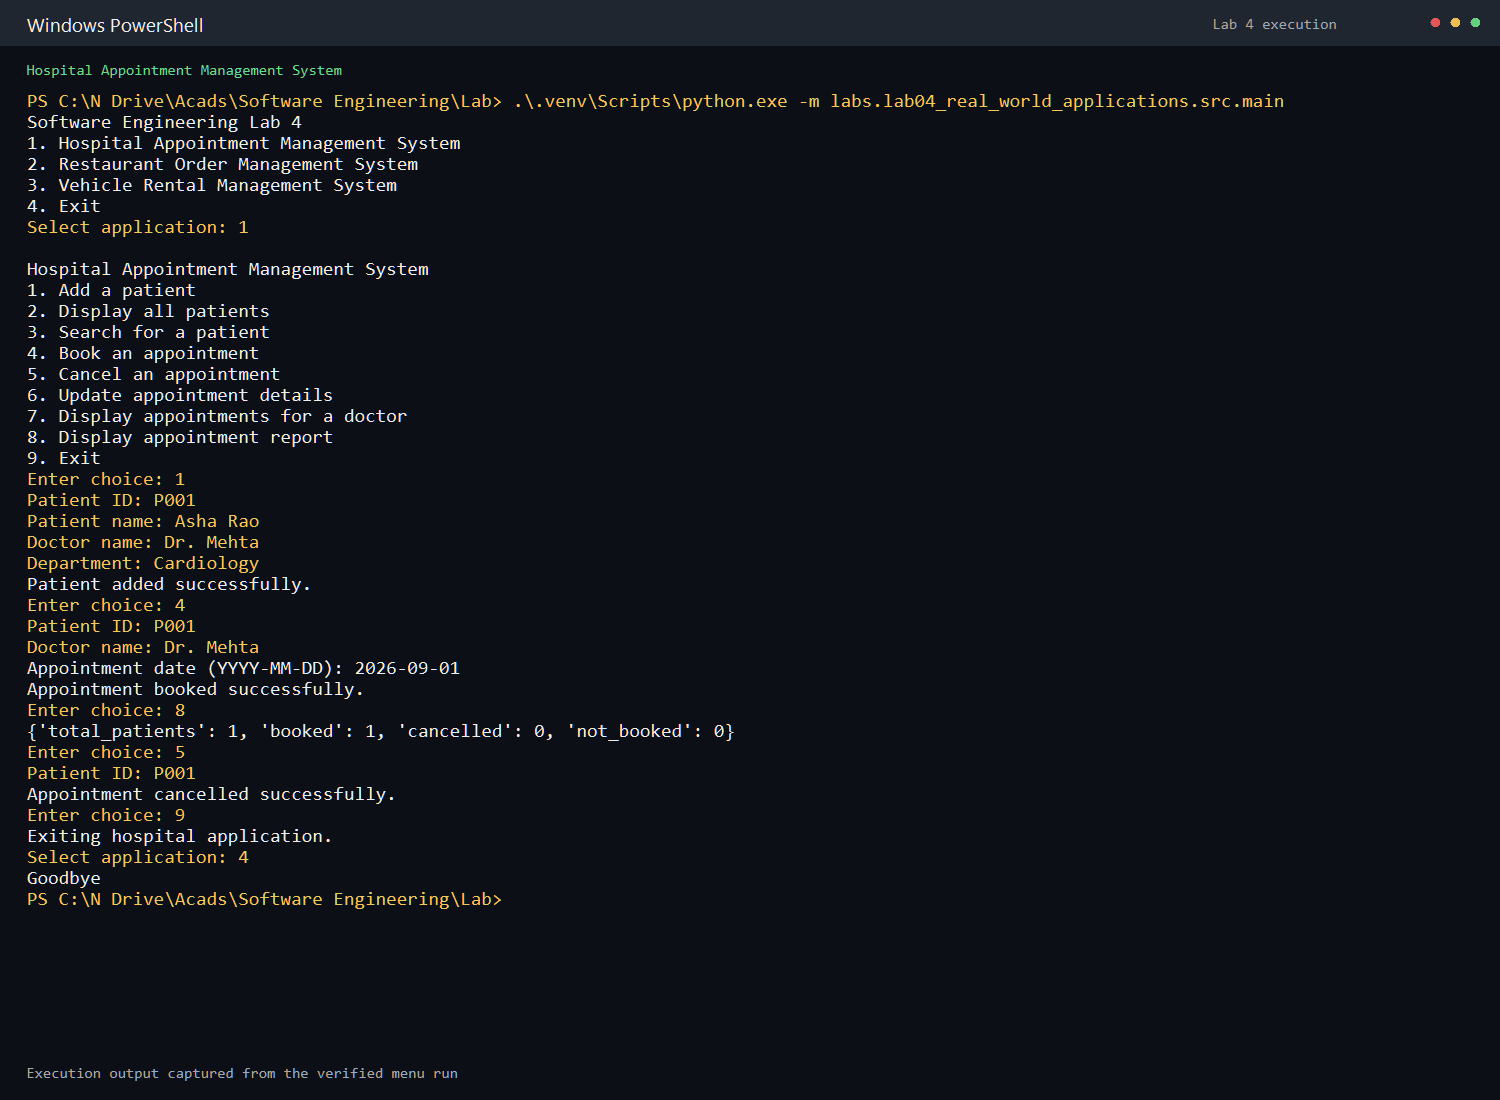
\includegraphics[width=0.92\linewidth]{screenshots/hospital_execution.png}
\begin{center}\textbf{Hospital appointment execution output}\end{center}

\clearpage
\vspace*{0.25in}
\noindent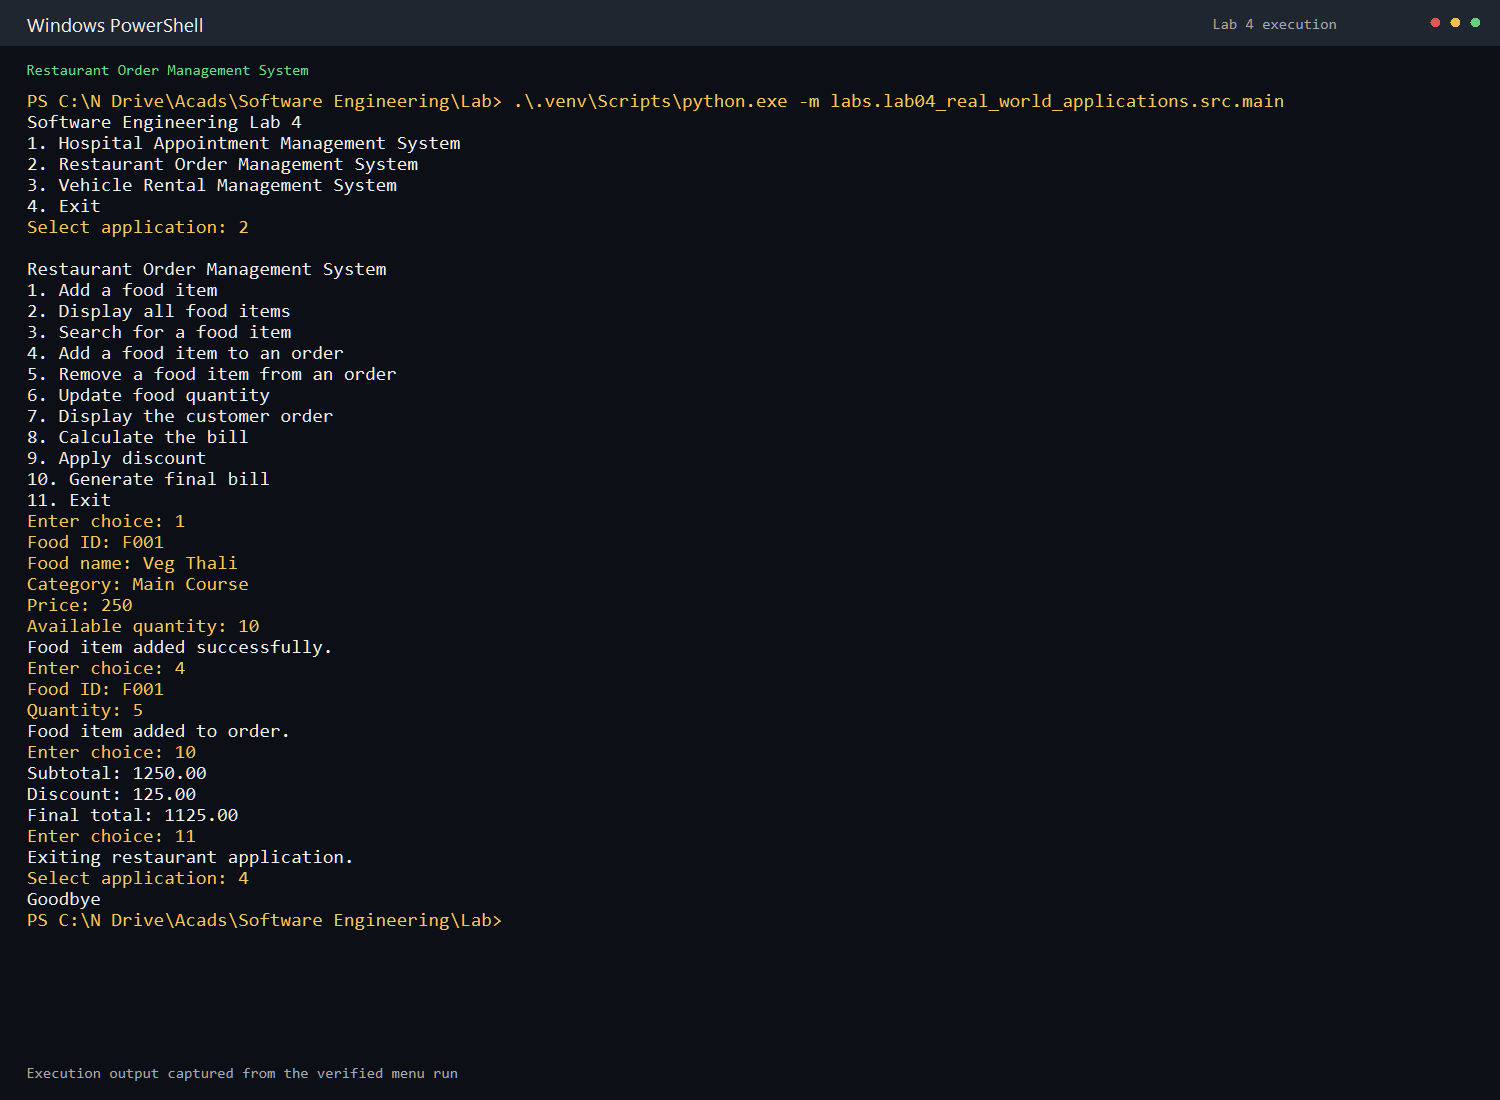
\includegraphics[width=0.92\linewidth]{screenshots/restaurant_execution.png}
\begin{center}\textbf{Restaurant order and bill execution output}\end{center}

\clearpage
\vspace*{0.25in}
\noindent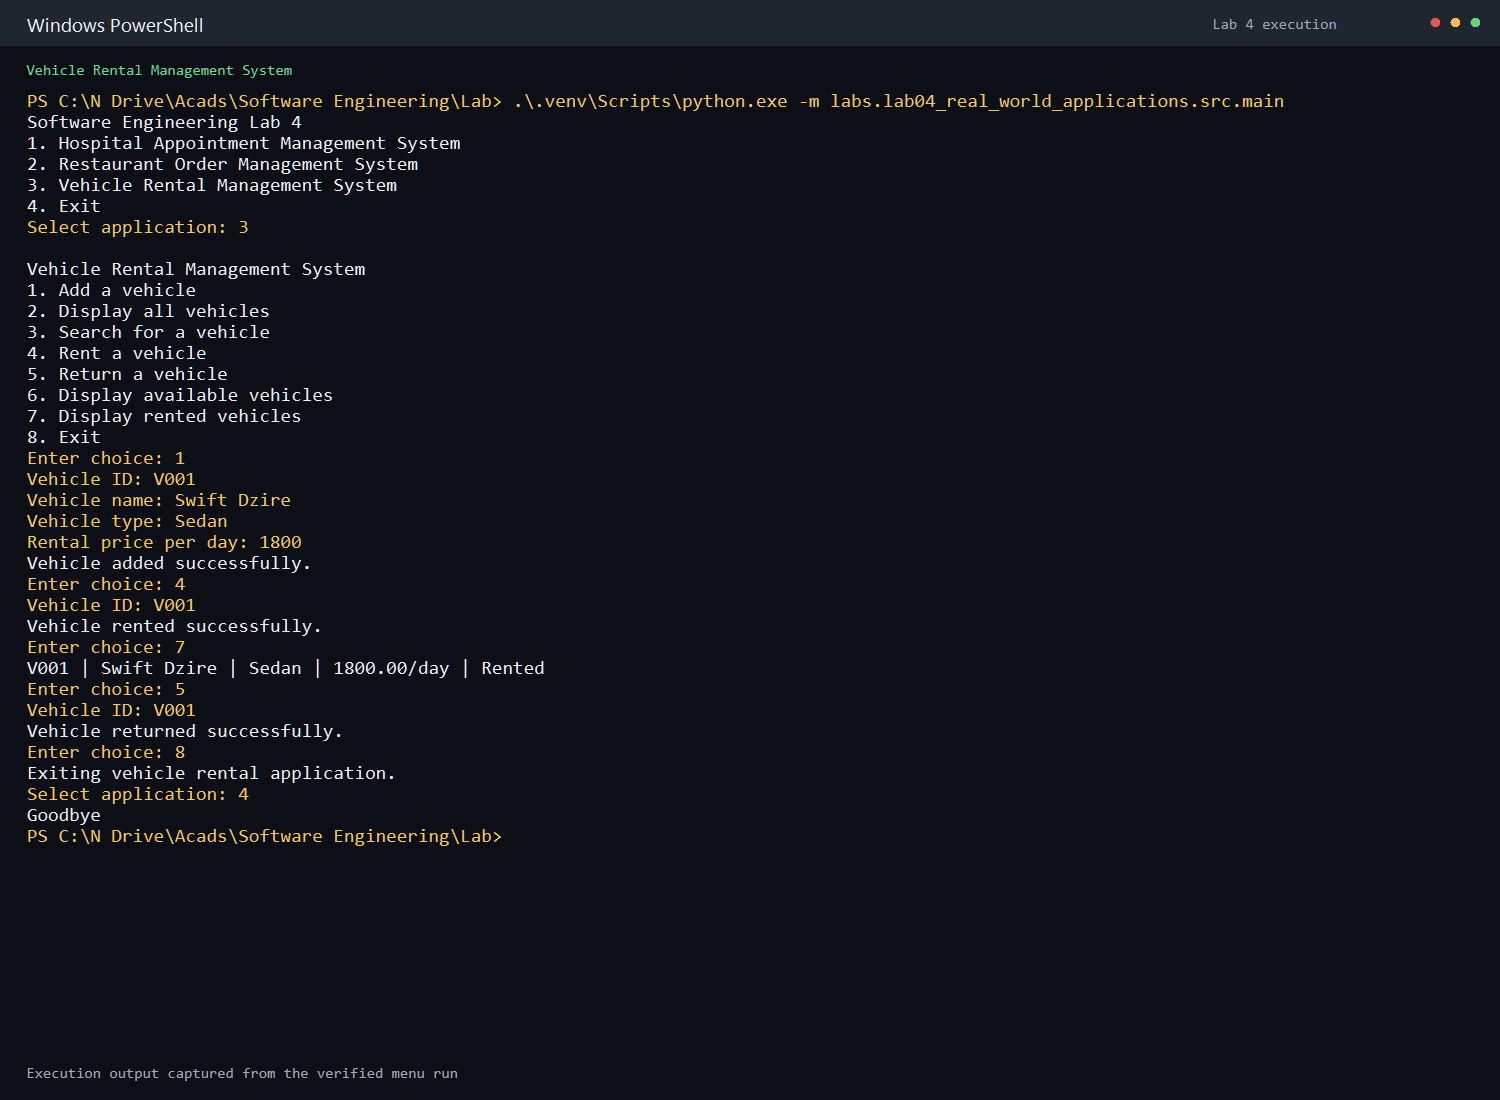
\includegraphics[width=0.92\linewidth]{screenshots/vehicle_execution.png}
\begin{center}\textbf{Vehicle rental execution output}\end{center}

\section{Submission Contents}
\begin{itemize}[leftmargin=*]
  \item Source code: \texttt{src/}
  \item Unit and integration tests: \texttt{tests/}
  \item Input data: \texttt{data/input/}
  \item Output files: \texttt{data/output/}
  \item Execution screenshots: \texttt{docs/screenshots/}
  \item Test specification: \texttt{docs/test\_specification.md}
  \item Editable test report: \texttt{docs/test\_execution\_report.md}
\end{itemize}

\section{Conclusion}
All three requested real-world applications were implemented as menu-driven
console programs. The applications include validation and error handling for
the required invalid scenarios, and the automated test suite confirms the main
business operations and menu behavior.

\end{document}
